\chapter{The Large Hadron Collider and the CMS detector\label{ch:cmsdetector}}

\section{The Large Hadron Collider}
The Large Hadron Collider (LHC)~\cite{LHC_CONCEPT} is a proton-proton collider currently being constructed at CERN, Geneva. It has been designed to achieve a centre-of-mass ($\sqrt{s}$) energy of 14\,~\TeV and an instantaneous luminosity of \hilumi. As well as colliding proton beams the LHC will also provide Heavy Ion (HI) collisions at a centre-of-mass energy of 1,312\,~\TeV and a luminosity of \hilumiHI.

Proton bunches are formed in the 26\GeV Proton Synchrotron (PS) with 25\,ns spacing. The beam will then be accelerated to 450\GeV by the Super Proton Synchrotron (SPS)~\cite{citeulike:821072} and transferred to the LHC ring. This process will be repeated 24 times, resulting in 2 counter-rotating beams each consisting of 2,808 bunches with a 25\,ns spacing and containing $1.15\times 10^{11}$ protons. Once circulating in the LHC, the bunches will be accelerated by 0.5\MeV/orbit by 1,232 r.f cavities until reaching 7\TeV.

The LHC will operate in a number of reduced modes over several years before reaching its design parameters. Initial commissioning will take place in the last few months of 2007 with beams consisting of just a few bunches. During this phase the r.f cavities will not be operational, limiting the beam energy to 450\,GeV from the SPS.

Following this the machine will be commissioned with 7\TeV beams. This will take approximately 5 months and will leave the 2nd half of 2008 for a pilot physics run. This pilot run will have a 75\,ns+ bunch spacing and a luminosity of \pilotlumi with the aim of taking 2--3\pbinv of data. 

Following the pilot run the first physics run will start in 2009 with a 75\,ns bunch spacing. An instantaneous luminosity of \lowlumi will be reached with an average of $\sim$5 inelastic collisions per bunch crossing. It is hoped that up to 5\fb of data can be collected during this period. 

The luminosity will be limited to \lowlumi until at least 2010 while the beam dump and collimation systems are staged. During this time the bunch spacing will be reduced from 75\,ns to 25\,ns with the aim of collecting 10--30\,\fb of data in the low luminosity r$\acute{e}$gime. After this the luminosity will increase and finally reach the design value, \hilumi, with 20 inelastic collisions each per bunch crossing.
%
%FIXME maybe move to last section
%These varying operational conditions result in several benchmark physics potential scenarios: 1\fbinv during initial operation, 10-30\fbinv during the ``low luminosity'' phase and 100-300\fbinv after several years of ``high luminosity'' running.
%%%%%

\section{The CMS detector}
The Compact Muon Solenoid (CMS)~\cite{CMS_LOI,CMS_TP} experiment is one of two general purpose detectors that will operate at the LHC. It has been designed to detect the widest range of new physics possible~\cite{CMS_TDR_PHYS_vol1, CMS_TDR_PHYS_vol2}. To facilitate this the main design goals were:
\begin{itemize}
\item Good muon identification;
\item Good charged particle tracking;
\item Good electromagnetic energy resolution; and
\item Good missing transverse energy (\MET) and jet resolution.
\end{itemize}

\begin{figure}[!htb]
  \centering
  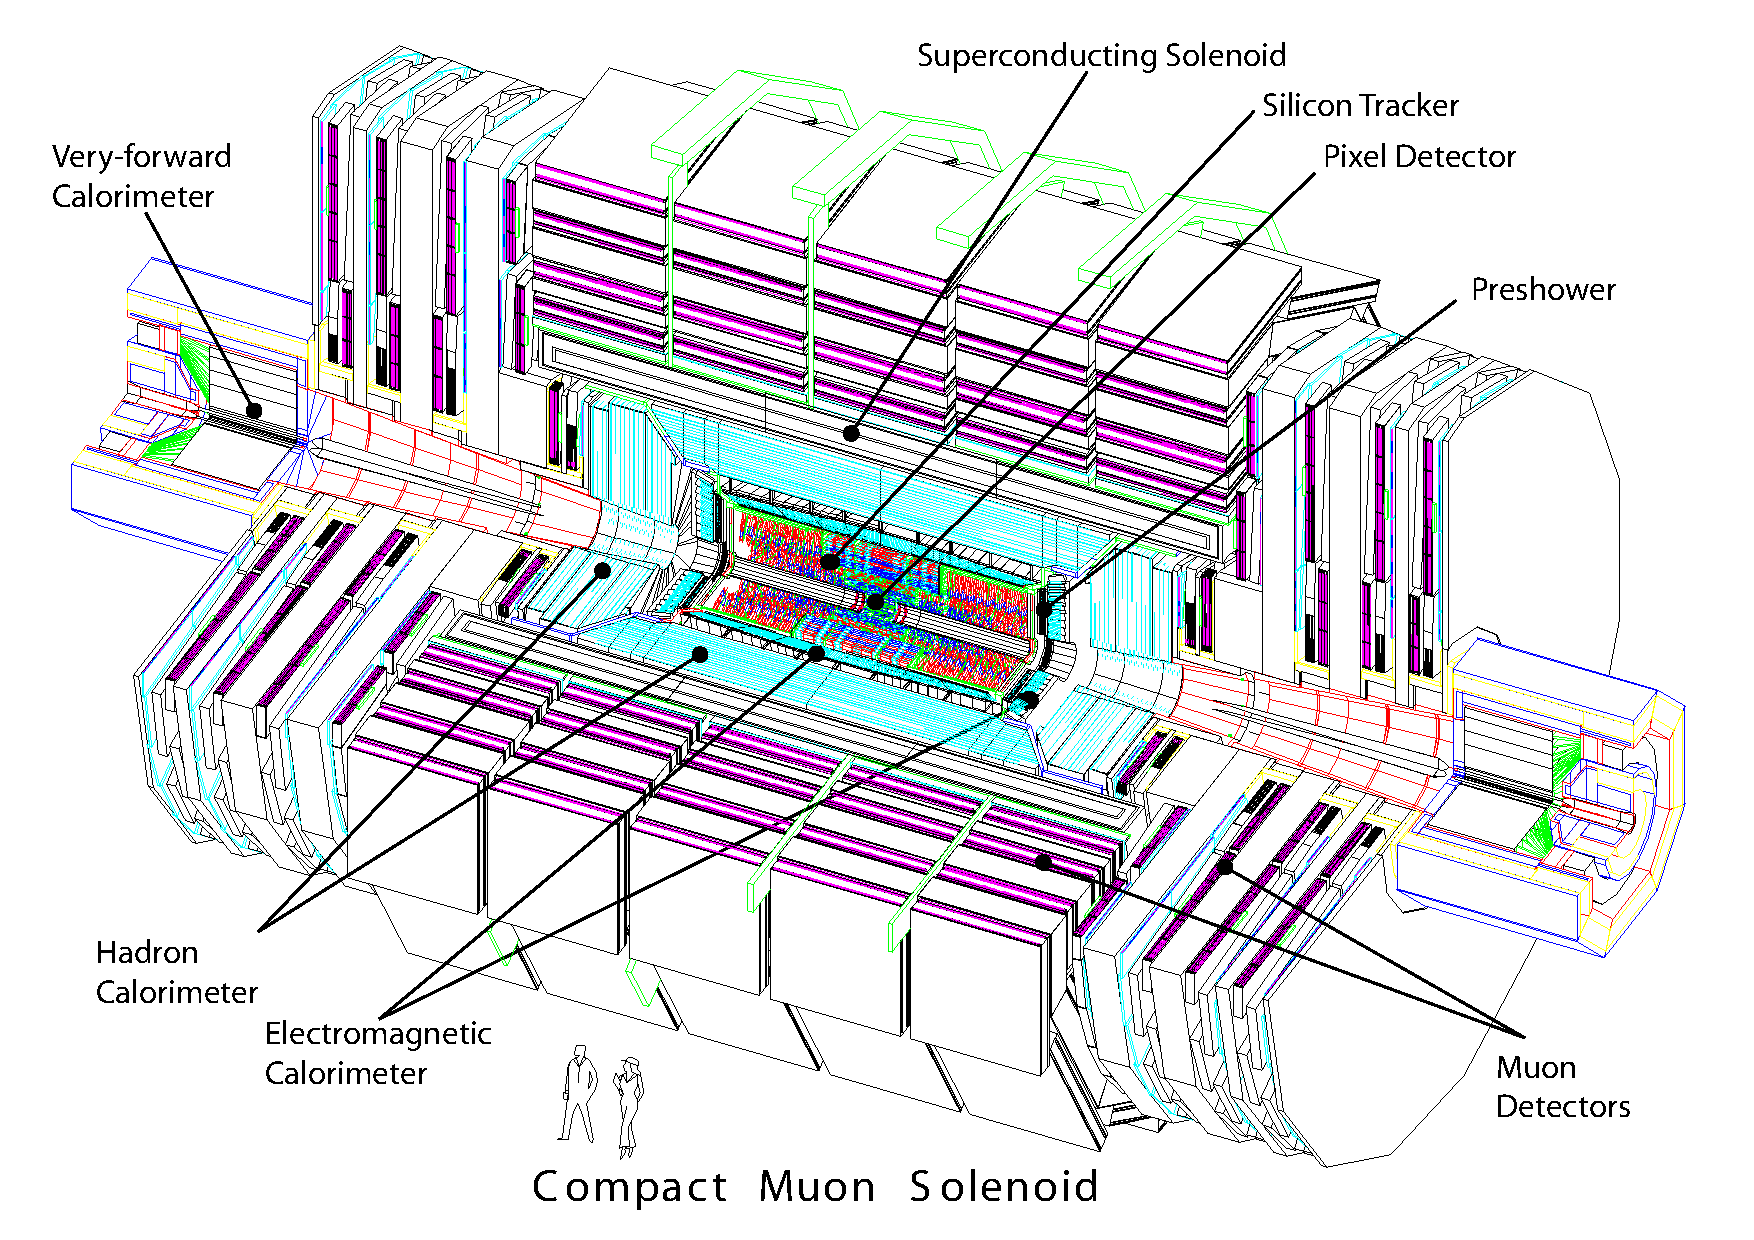
\includegraphics[width=0.95\textwidth]{cms/cms_complete_labelled}
  \caption{An exploded view of the CMS detector showing the major components.~\cite{CMS_TDR_PHYS_vol1}
  \label{fig:cms}}
\end{figure}

CMS, shown in Figure~\ref{fig:cms}, is a large and complex detector composed of multiple subsystems and detectors. Major sub-detectors include a silicon tracking detector~\cite{CMS_TRKTDR}, a crystal electromagnetic calorimeter~\cite{CMS_ECALTDR}, scintillating hadronic calorimeter~\cite{CMS_HCALTDR} and several muon detectors~\cite{CMS_MUONTDR}. The CMS detector is 21.6\,m long, has a diameter of 14.6\,m, weighs 12,500 metric tons and has $\sim\,10^{8}$ electronic readout channels. 

Charged particle momentum measurement is provided by the bending power of a 4T magnetic field. Provided by a 13 m long, 5.9 m diameter superconducting solenoid coil~\cite{CMS_MAGTDR}. The coil current is 19.5 kA giving a total stored energy of 2.7 GJ. The magnetic flux is returned by a 1.8 m thick iron return yoke. The tracking and calorimetry systems are enclosed within the coil and the return yoke is instrumented with the muon detectors.

\subsection{CMS coordinate system}
In the CMS coordinate system the origin is centred on the nominal interaction point with the x-axis pointing radially inward towards the centre of the LHC ring, the y-axis pointing vertically upward and the z-axis pointing along the beam direction towards the Jura mountains. The azimuthal angle, $\phi$, is measured from the x-axis in the x-y plane. The polar angle, $\theta$, is measured between the line connecting the coordinate to the interaction point and the z-axis. Pseudorapidity, $\eta$, is defined as $\eta=-\ln\tan(\theta/2)$. Distance in the $\phi - \eta$ plane is measured as $\mathrm{\Delta R = \sqrt{\Delta \eta^{2} + \Delta \phi^{2}}}$

Momenta and energy measured transverse to the beam, \PT and \ET respectively, are computed from their x and y components (i.e. \ET = $\mathrm{E_x + E_y}$). The energy imbalance measured in the transverse plane is denoted by \MET, where $\MET = -\ET$.

\subsection{The Silicon Tracker}

\begin{figure}[tb]
  \centering
  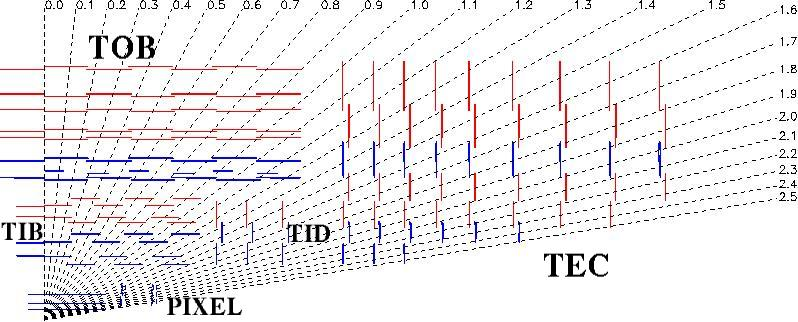
\includegraphics[width=0.95\textwidth]{cms/tk_layout}
  \caption{A one-quarter view of the tracker, showing all silicon detector layers. See the text for a description of the acronyms. Red (blue) layers use single (double) sided modules with dashed lines showing the pseudorapidity. From~\cite{CMS_TDR_PHYS_vol1}.
  \label{fig:tracker}}
\end{figure}

\begin{figure}[tb]
  \centering
  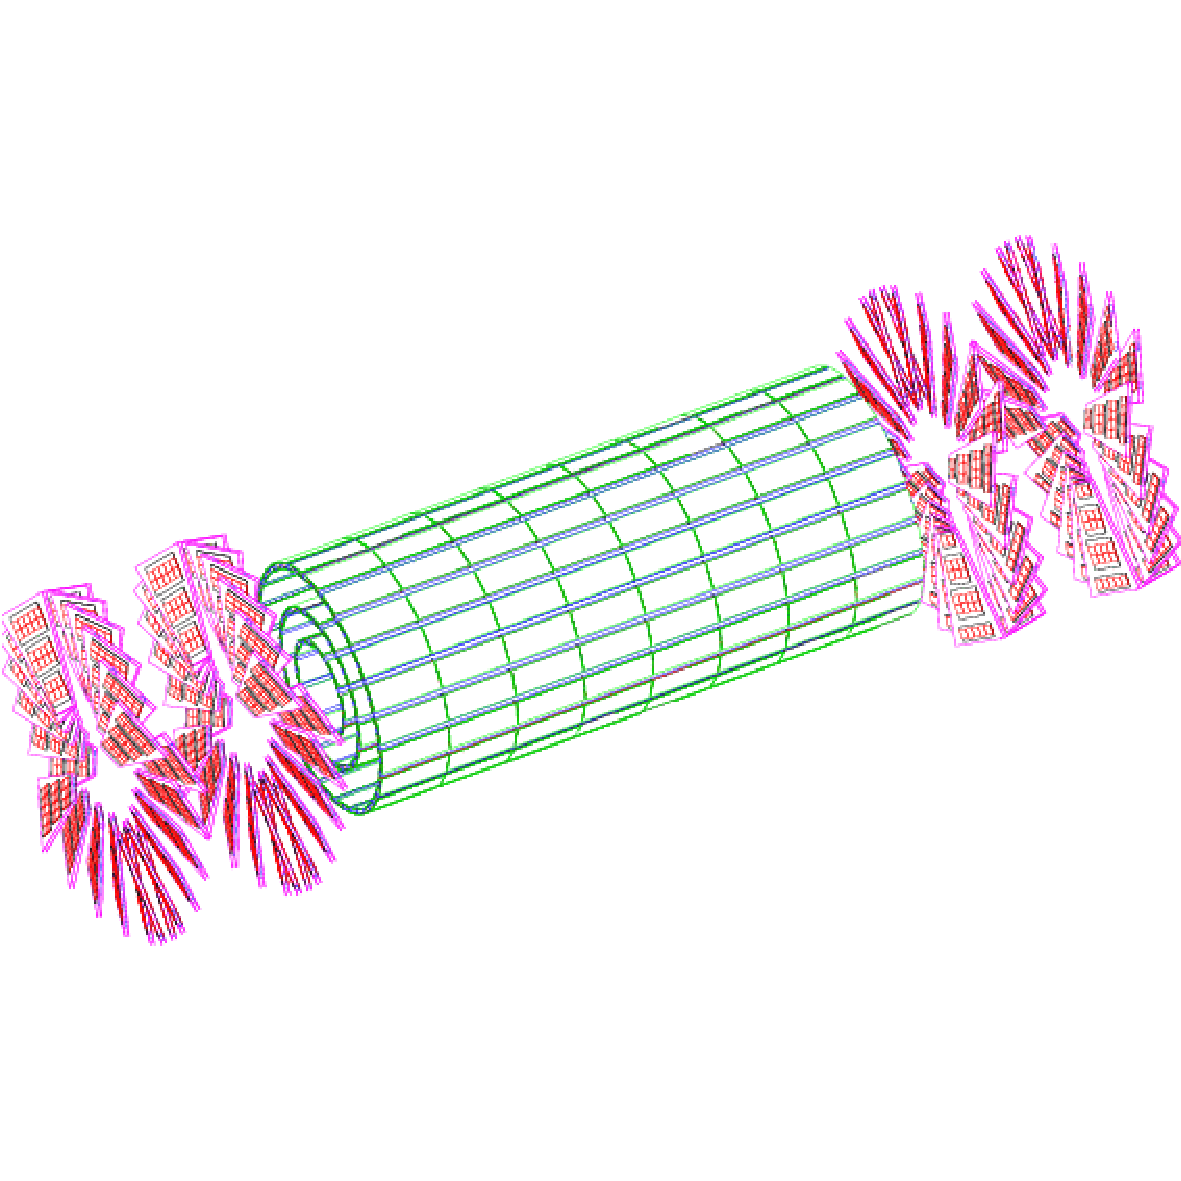
\includegraphics[width=0.8\textwidth]{cms/3l_2disk_70_0_20}
  \caption{Layout of pixel detectors in the CMS tracker.~\cite{CMS_TDR_PHYS_vol1}\label{fig:pixels}}
\end{figure}

The closest sub detector to the interaction point is the silicon tracking system. It measures the trajectories and momenta of charged particles up to $|\eta| \lesssim 2.4$. CMS has opted for a full silicon tracker providing a relatively low number of precise measurement points instead of a continuous tracking technology. Two different silicon technologies are used: pixel and microstrip detectors. Close to the beam pipe the high particle flux requires small pitch pixel detectors whereas further out the occupancy drops sufficiently to allow silicon microstrip detectors to be used. The tracker, shown in Figure~\ref{fig:tracker}, has an outer radius of 110 cm, is 540 cm long and has $\sim44\times10^{6}$ readout channels. 

The pixel detector, shown in Figure~\ref{fig:pixels}, consists of 3 barrel layers with 2 pairs of endcap disks and provides two hit coverage up to $|\eta| = 2.2$. The barrel layers are located at radii of 4.4\,cm, 7.3\,cm and 10.2\,cm and are 53\,cm long. The two endcap disks are located at $|z| = 34.5$ cm and 46.5\,cm with radii of 6\,cm to 15\,cm.

In order to maximise the vertex resolution the pixel pitch is $\approx100~\times150~\mmsquare$. The pixel spatial resolution is increased by using analogue signal interpolation of the charge sharing induced by the large Lorentz drift in the magnetic field. Thus the barrel pixel layers are collinear to the beam and the endcaps are arranged in a turbine-like geometry with blades rotated by 20\de. The spatial resolution is 10\micron in r-$\phi$ and 20\micron in z giving a vertex resolution of $\sim40\,\micron$.

The silicon strip tracker surrounds the pixel detector and covers the range $|\eta| < 2.4$. The strip tracker is split into 2 systems, inner and outer, each of which has barrel and endcap sections. Most detector layers utilise single sided microstrips but some use ``stereo'' modules consisting of two tilted back-to-back modules which provide a 3D hit measurement. The modules used in the various parts of the silicon tracker are listed in Table~\ref{tab:intro:tracker}.

\begin{table}[!h]
\centering
\begin{tabular}{lrrr}
\hline
part & No. detectors  & thickness $(\micron)$ & mean pitch $(\micron)$\\
\hline
TIB & 2724& 320 & 81/118     \\
TOB & 5208& 500 & 81/183     \\
TID & 816& 320 & 97/128/143     \\
TEC & 2512& 320 & 96/126/128/143     \\
TEC(2) & 3888& 500 &  143/158/183    \\
\hline
\end{tabular}
\caption{Detector types in the silicon tracker. See text for an explanation of the acronyms.~\cite{CMS_TDR_PHYS_vol1} \label{tab:intro:tracker}}
\end{table}

The Tracker Inner Barrel (TIB) is composed of 4 microstrip layers covering $|z| <$ 65\,cm, where the first 2 layers use stereo modules with a stereo angle of 100\,mrad. The silicon sensors have a thickness of 320\micron and a length of 10\,cm. Point resolutions of 23--34\micron in r-$\phi$ and 230\micron in z are obtained depending on the layer. Each inner endcap, Tracker Inner Disk (TID), has three microstrip layers, the first two of which have stereo modules. The microstip detectors are 320\micron thick with a minimum length of 10 cm. A point resolution of 23--34\micron in r-$\phi$ and 230\micron in z is obtained.

The outer barrel system, Tracker Outer Barrel (TOB), comprises 6 layers covering the range $|z| <$ 110 cm with the first two layers using stereo modules. The point resolution varies from 35--52\micron in r-$\phi$ and is constant at 530\micron in z. The Tracker EndCaps (TEC) comprise 9 layers over the range $120 < |z| < 280$ cm. The first two and the fifth disks have stereo modules. The microstrips have a thickness of 320--500\micron and a length of 25\,cm. A point resolution of 35--52\micron in r-$\phi$ and 530\micron in z is obtained.

%each comprised of a barrel and 2 endcap systems. The Tracker Inner Barrel (TIB) comprises 4 layers of microstrips while each endcap, Tracker Inner Disk (TID), has 3 layers

%with 2 endcap systems, Tracker Inner Disks (TID). The barrel section comprises 4 layers of microsrips while the endcaps have 3 layers. The 
%The Tracker Inner system comprises of a barrel section with 4 layers of microstrips (TIB), while the encap (TID) system includes 3 endcap disks on either side    while the encaps are ith 3 endcap disks, Tracker Inner Disks (TID), on each side. 
%microstip detectors have a minimum cell size of 10cm\times80$\mu$m and provide a point resolution of $23-34\mu m$ in r-$\phi$ and 230$\mu m$ in z. 

%The outer system 
%The Tracker Outer Barrel (TOB) comprises 6 layers with 9 endcap disks at each end. These microstrips are larger with a maximum cell size of 25cm\times180$\mu$m giving a resolution of $35-52\mu m$ in r-$\phi$ and 530$\mu m$ in z.

\begin{figure}[htb]
  \centering
  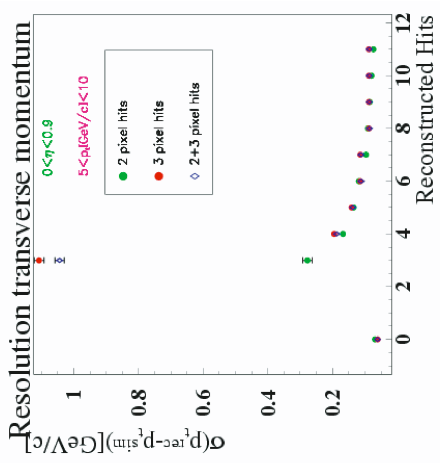
\includegraphics[width=0.45\textwidth,angle=-90]{cms/pt_perf_hits}
  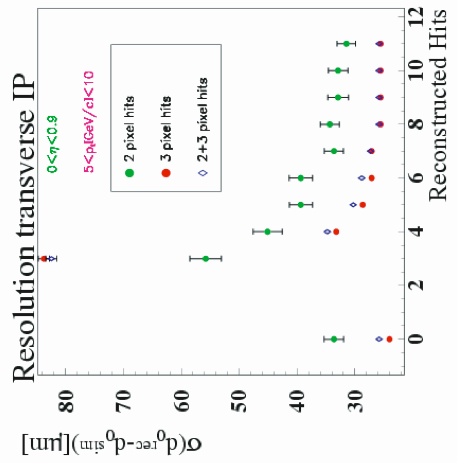
\includegraphics[width=0.45\textwidth,angle=-90]{cms/d0_perf_hits}
  \caption{The tracker \PT (left) and transverse impact parameter, d0, (right) resolution as a function of the number of reconstructed tracker hits.}
  \label{fig:tracker_perf_hits}
\end{figure}

\begin{figure}[htb]
  \centering
  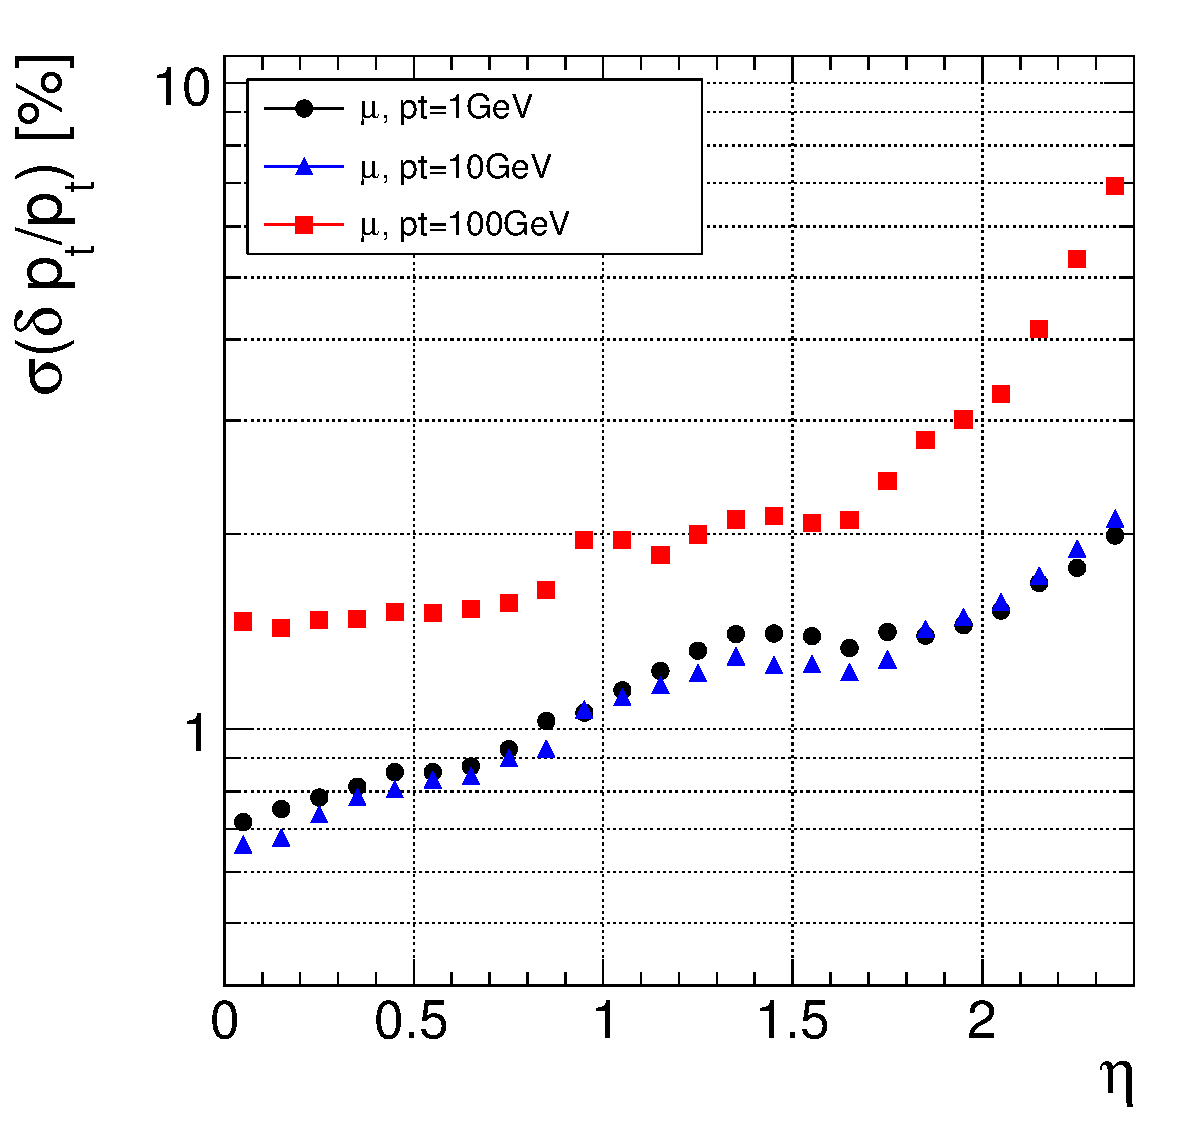
\includegraphics[width=0.45\textwidth]{cms/muon_all_pt-col}
  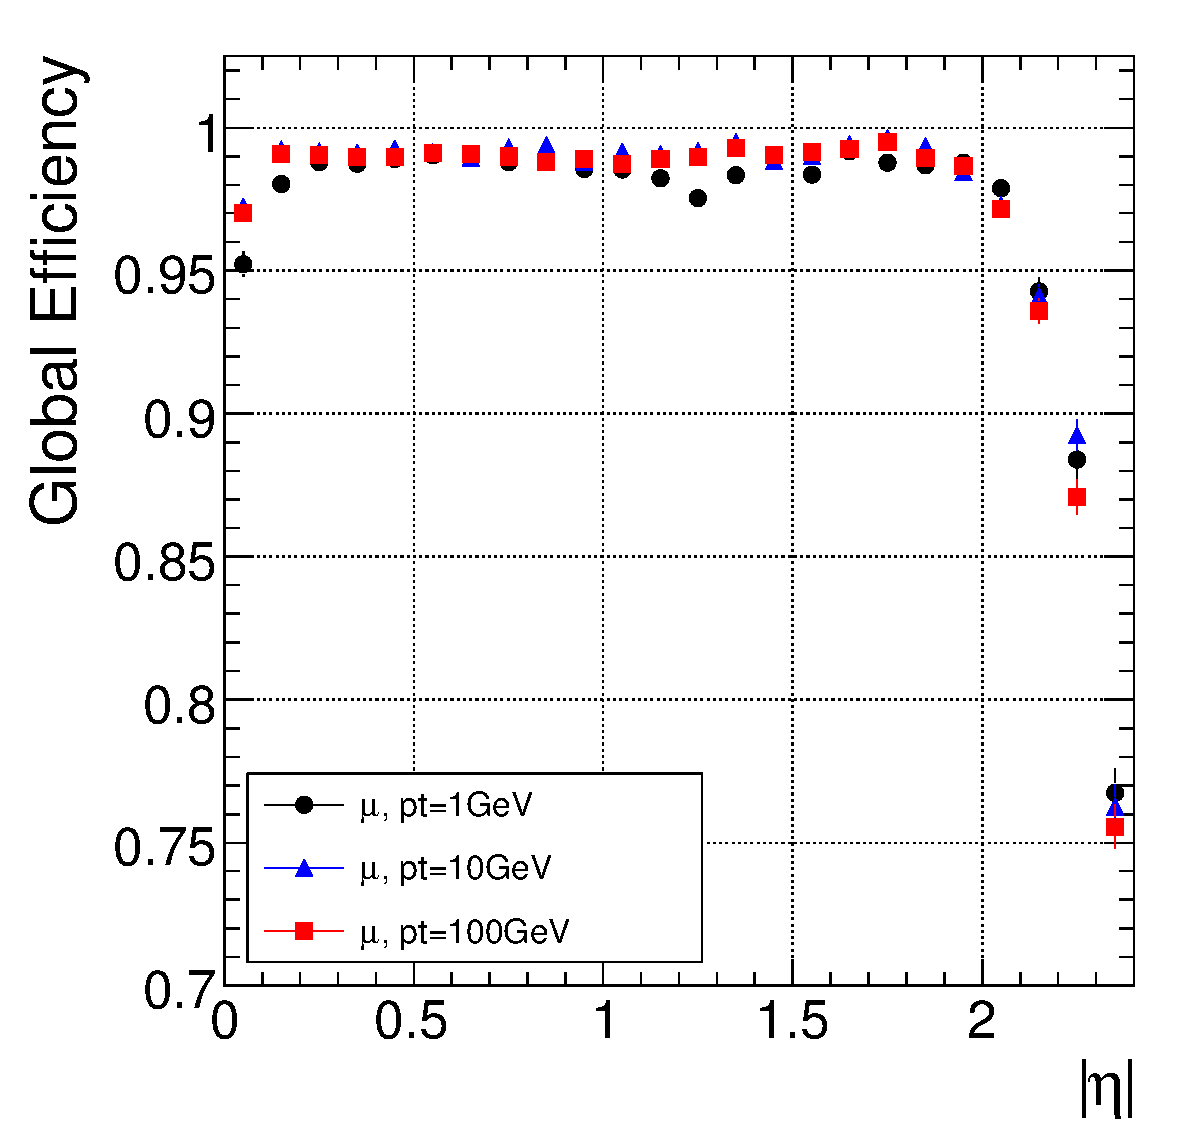
\includegraphics[width=0.45\textwidth]{cms/muonGlobalEff-col}
  \caption{Tracker performance for muons with transverse momenta of 1, 10 and 100\GeVc: transverse momentum resolution (left) and global track reconstruction
efficiency (right).~\cite{CMS_TDR_PHYS_vol1}
  \label{fig:tracker_perf}}
\end{figure}

Figure~\ref{fig:tracker_perf_hits} shows the tracker performance as a function of the number of reconstructed hits. It can be seen that performance with only the pixel layers operational is reduced. Operating in this mode is significantly quicker than using the full tracker due to the reduced number of read out channels and combinatorials and is used for triggering when less precise but fast measurements are required.

Figure~\ref{fig:tracker_perf} shows the tracker \PT resolution and global tracking efficiency for muons with \PT of 1, 10 and 100 \GeVc. Global efficiency is defined as the reconstruction efficiency for all tracks, taking into account tracker acceptance, hit efficiency and pattern recognition efficiency. The \PT resolution can be parameterised:

\begin{equation}
\frac{\sigma_{\PT}}{\PT} = a\PT \oplus 0.5\%
\label{eqn:TRK_perf}
\end{equation}

with \PT in \TeV and a = 15 for $|\eta| < 1.6$ and 60 for $1.6 < |\eta| < 2.5$~\cite{CMS_TDR_PHYS_vol1}.

\subsection{The Electromagnetic Calorimeter}
Surrounding the silicon tracker is the electromagnetic calorimeter (ECAL). The ECAL is divided into a barrel and 2 endcap sections, shown in Figure~\ref{fig:ECAL}. CMS has chosen scintillating lead tungstate (PbW$\mathrm{O_{4}}$) crystal to provide precise electron and photon energy measurement. Lead tungstate crystals are radiation hard, have short radiation lengths ($X_{0}=0.89$ cm) and are fast (80\% of light is emitted within 25 ns). This choice allowed a fast, fine grained and compact ECAL which could be placed inside the coil. PbW$O_{4}$ crystals yield a relatively low number of photons (30$\gamma$/\MeV) and so need to be read out by  photodetectors with an intrinsic gain as photo multipliers cannot operate in the high magnetic field.

\begin{figure}[htb]
  \centering
  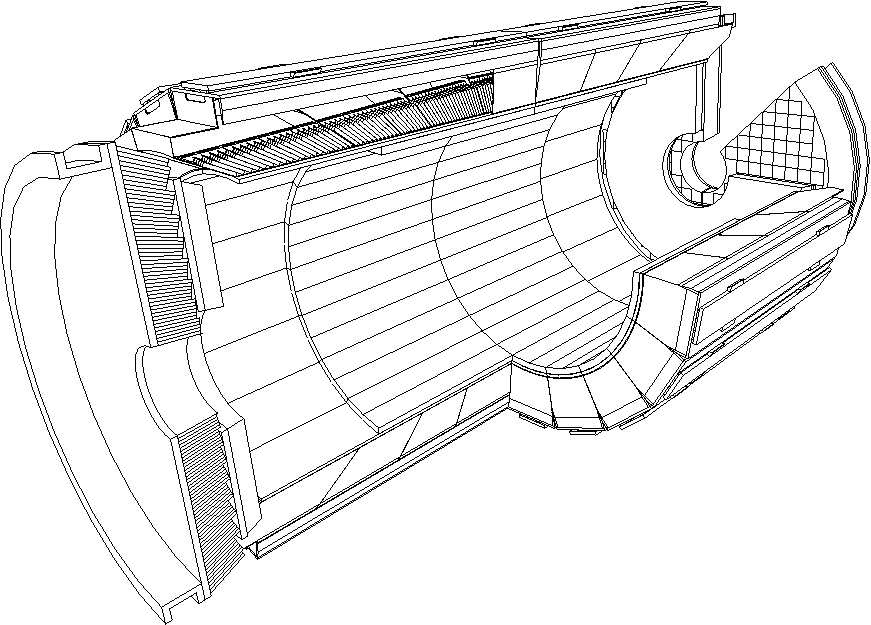
\includegraphics[width=0.85\textwidth]{cms/ECAL}
  \caption{A 3D view of the CMS electromagnetic calorimeter.~\cite{CMS_ECALTDR}}
  \label{fig:ECAL}
\end{figure}

The ECAL barrel (EB) begins at a radius of 129\,cm and covers the range $|\eta| < 1.479$. 61,200 crystals are grouped together to form one of 36 identical ``supermodules''. Each supermodule covers half of the barrel length. The crystals are mounted 3\de off axis from the nominal vertex position to avoid energy leakage between crystals. Each crystal measures $22~\times22~\times230\,\mmtriple$ (25.8 $X_{0}$) and covers an area of $\Delta\eta\times\Delta\phi = 0.0174\times0.0174$. These crystals are read out by silicon avalanche photodiodes (APDs) with a gain of 50. 

The ECAL endcaps (EE) are located 314\,cm from the vertex and cover the range $1.479 < |\eta| < 3.0$. Each endcap is constructed from two ``Dees'' consisting of semi-circular aluminium plates mounting crystals in groups of $5\times5$ crystals, known as ``supercrystals''. The endcaps crystals are tilted off axis in an x-y grid. A total of 21,528 crystals of dimensions $28.6\times28.6\times220~\mmtriple$ (24.7 $X_{0}$) are used in the endcaps. Vacuum phototriodes are used for the endcap readout as they are more radiation hard than APDs.

A preshower detector comprised of two planes of lead absorber followed by silicon strip detectors is placed in front of the endcaps, covering $1.48 < |\eta| < 2.6$. These are used to help identify neutral pions in the endcap region where the average pion energy is high enough to make resolving individual photons difficult given the calorimeter granularity.

The ECAL performance has been evaluated in a test beam~\cite{CMS_TDR_PHYS_vol1}. High energy electrons ($20 \le \ET \le 250 \GeV$) were used with a full barrel supermodule. The measured electron energy resolution is shown in Figure~\ref{fig:ECAL_perf}. The resolution can be parameterised as 

\begin{equation}
	\frac{\sigma}{E} = \frac{3.63\%}{\sqrt{E}} \oplus \frac{0.124\%}{E} \oplus 0.26\%,
\label{eqn:ECAL_perf}
\end{equation}

where E is the beam energy in \GeV, the first term is the stochastic term, the second the noise and the third the constant term. The Stochastic term comes from fluctuations in lateral containment and photostatistics~\cite{CMS_TDR_PHYS_vol1}, the noise term originates from preamplifier, digitisation and pileup noise, and the constant term comes from energy leakage and inter-crystal calibration.

\begin{figure}[tb]
  \centering
  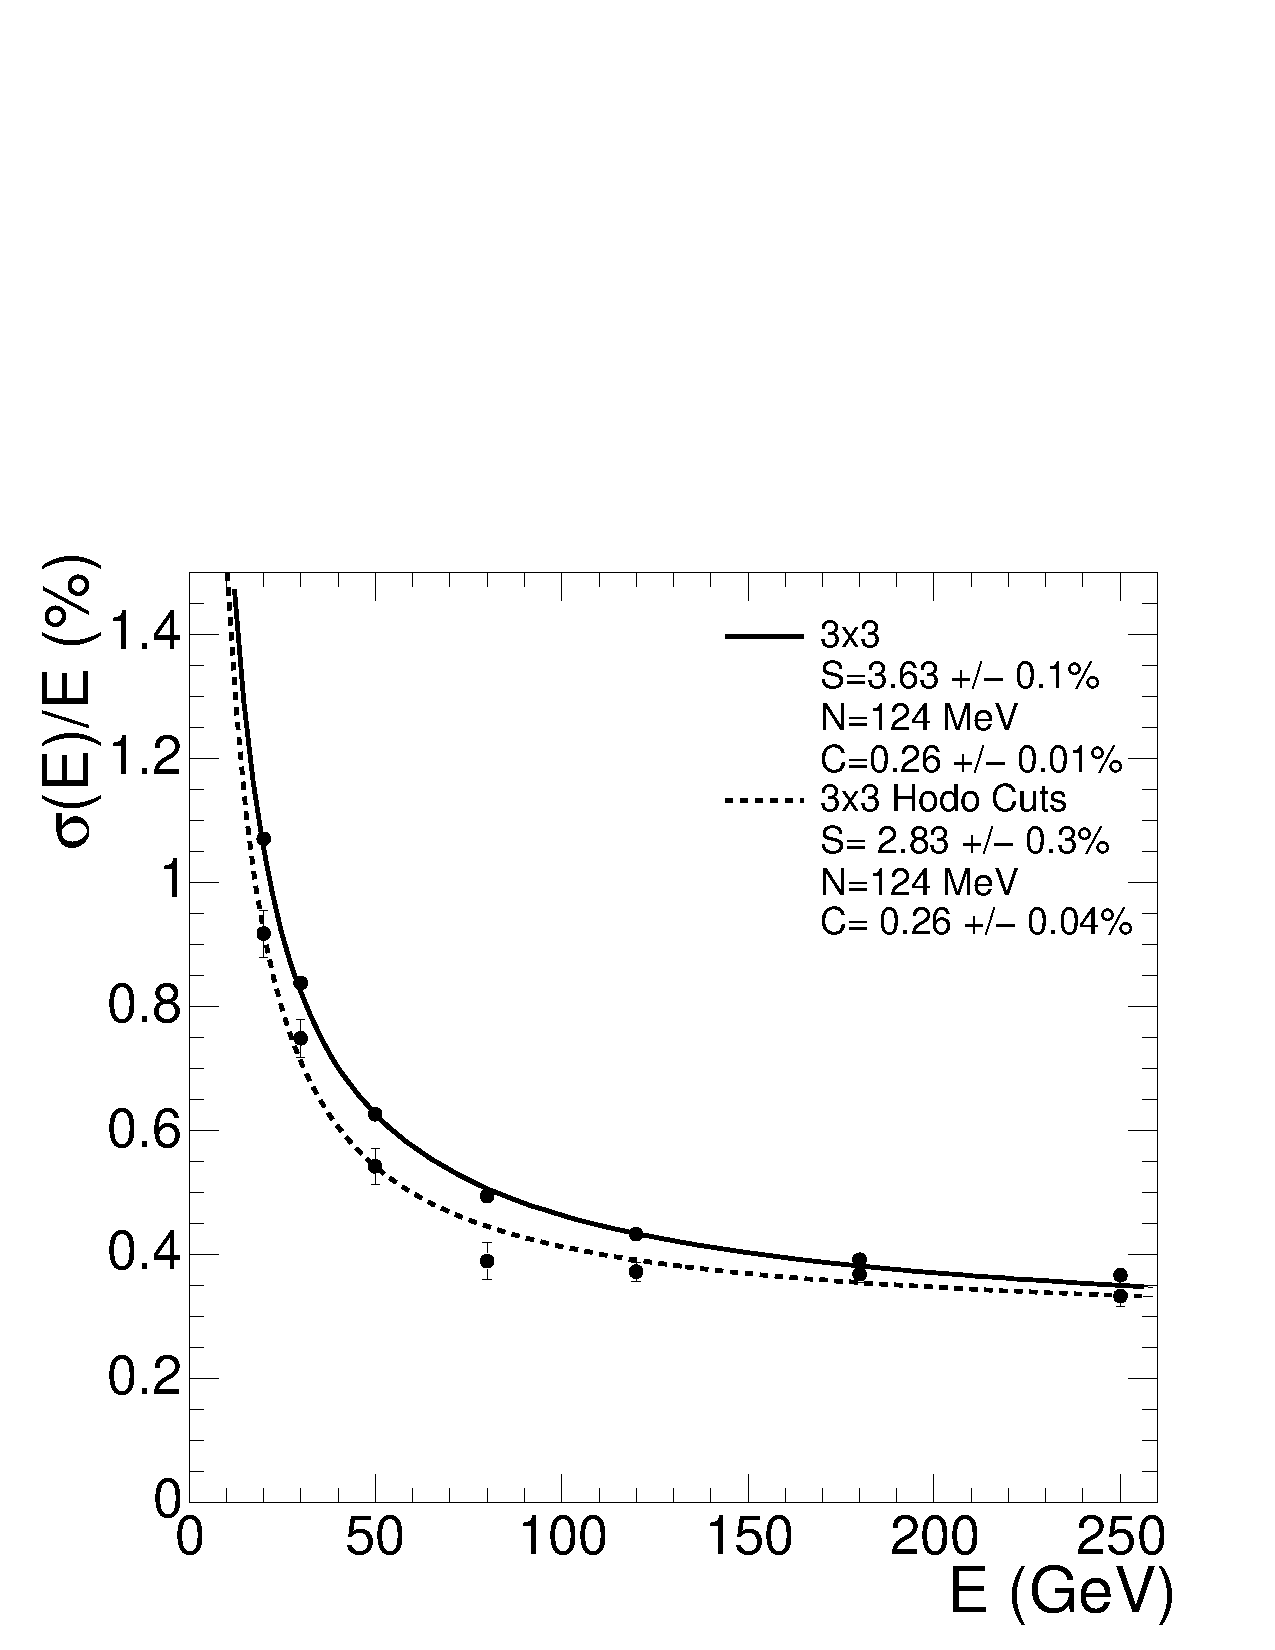
\includegraphics[width=0.55\textwidth]{cms/Resolution_Comp_Hodo_3x3_704_tdr}
  \caption{ECAL electron test beam data energy resolution as measured by an array of 3$\times$3 crystals. The upper (lower) series shows events taken with a 20$\times$20 (4$\times$4)\,~\mmsquare trigger. The fit parameters correspond to those in Equation~\ref{eqn:ECAL_perf}.~\cite{CMS_TDR_PHYS_vol1}
  \label{fig:ECAL_perf}}
\end{figure}


%%%%%
%These are used for neutral pion rejection by resolving the individual photons in the decay. A preshower is not needed for the barrel as the average pion energy in this region is low resulting in a large opening angle between the two photons. Which together with the granularity of the crystal detector alow both to be resolved.
%%%%%

\subsection{The Hadronic Calorimeter}
Surrounding the electromagnetic calorimeter is the hadronic calorimeter (HCAL). In order to minimise non-Gaussian energy resolution tails and to provide good containment the HCAL was placed inside the magnet coil. This required a compact absorber and left little room for the active medium. Brass was chosen for the absorber because it is non-magnetic and has a short interaction length ($\lambda$). Tile/fibre technology was chosen for the active medium together with wavelength-shifting fibre readouts. 

The barrel section, denoted HB, spans the region $|\eta| < 1.4$ and is read out in towers of $\Delta\eta \times \Delta\phi = 0.087\times0.087$ in a single longitudinal sampling. The HB has 15 brass plates comprising 6.5\,$\lambda$ thus additional layers, known as the hadron outer (HO), are placed behind the coil, hadron outer (HO), to act as a tail catcher. This covers the region $|\eta| < 1.26$ and uses the same tower geometry as the barrel. The HO extends the barrel HCAL depth to over 10\,$\lambda$.
 
Hadron endcap (HE) disks are located either side of the solenoid coil and span the region $1.3 < |\eta| < 3.0$ with towers varying in size from $\Delta\eta \times \Delta\phi = 0.087\times0.8 - 0.35\times0.8$.

To extend the $\eta$ coverage, a forward calorimeter, hadron forward (HF), is located at the edges of CMS covering the region $3.0 < |\eta| < 5.0$ (see Figure~\ref{fig:cms}). This detector is constructed from steel and quartz fibre. These materials lead to shorter and narrower jets which is useful in the high flux forward region.

\begin{figure}[tb]
  \centering
    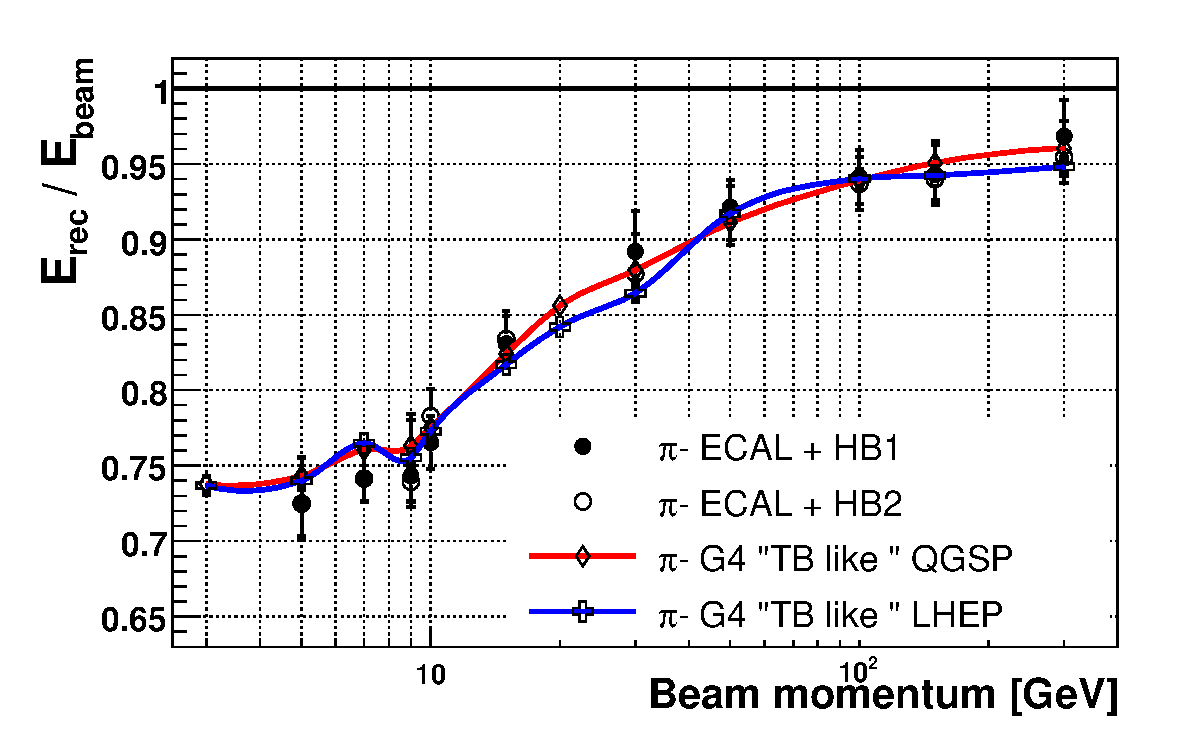
\includegraphics[width=0.48\textwidth]{cms/linearity5-300}
    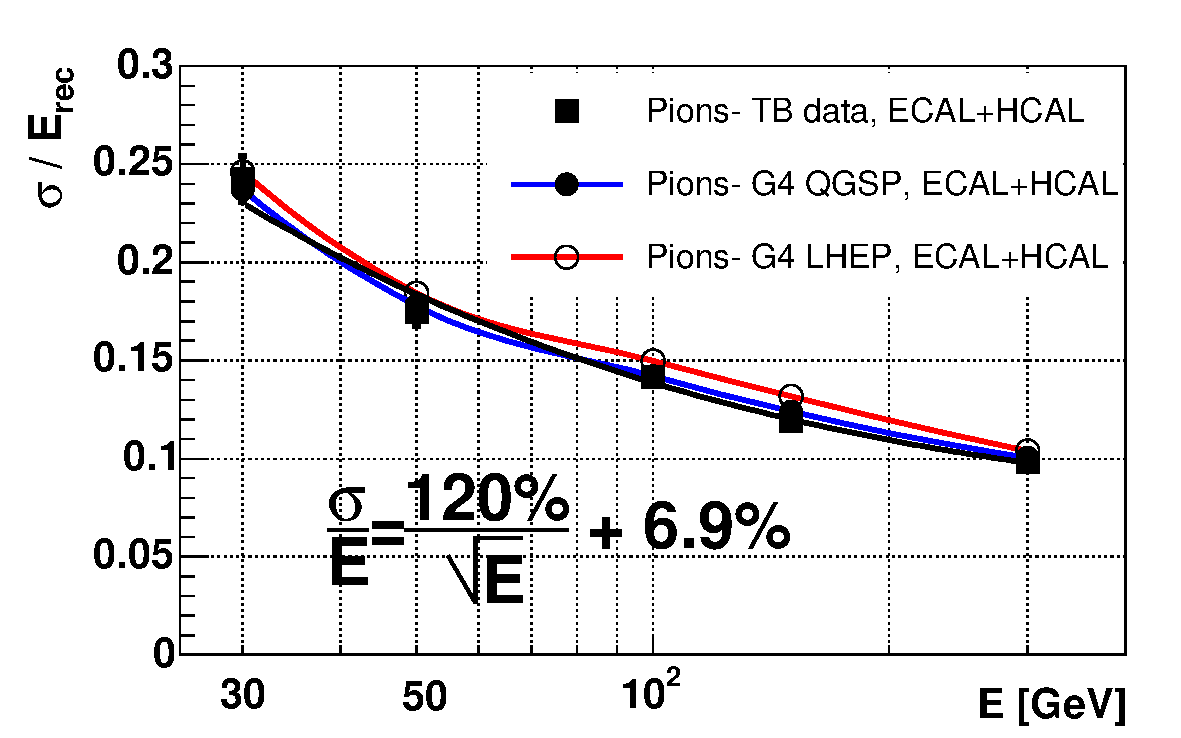
\includegraphics[width=0.48\textwidth]{cms/res_fit}
    \caption{Nominal raw energy response and fractional energy resolution 
as a function of ECAL+HB energy for \piminus. The fit for the non-compensated
energy resolution is shown. Results for both testbeam and simulated (labeled G4) data are shown.~\cite{CMS_TDR_PHYS_vol1}}
    \label{fig:HCALparticle}
\end{figure}

Test beams have been used to evaluate the HCAL performance and characteristics. The 2004 HCAL test beam used a replica of a slice through the CMS detector with a \piminus beam~\cite{CMS_TDR_PHYS_vol1}. The prototype detector included an aluminium slab, representing the solenoid, a prototype ECAL detector and 144 HB and 60 HO towers. This detector was exposed to \piminus beams of energies 2-9~\GeV and 10-300~\GeV. The single particle energy response and resolution are shown in Figure~\ref{fig:HCALparticle} both for test beam and simulated data. The energy resolution can be parameterized as:

\begin{equation}
	\frac{\sigma}{E}= \frac{120\%}{\sqrt{E}} \oplus 6.9\%
\end{equation}

The HCAL jet and \MET performance have been evaluated with simulated QCD multi-jet events at \lowlumi~\cite{CMS_TDR_PHYS_vol1}. The jet energy response for jets of various generated \ET (\ETMC) is shown in Figure~\ref{fig:jet_scale}.

\begin{figure}[bt]
   \centering
    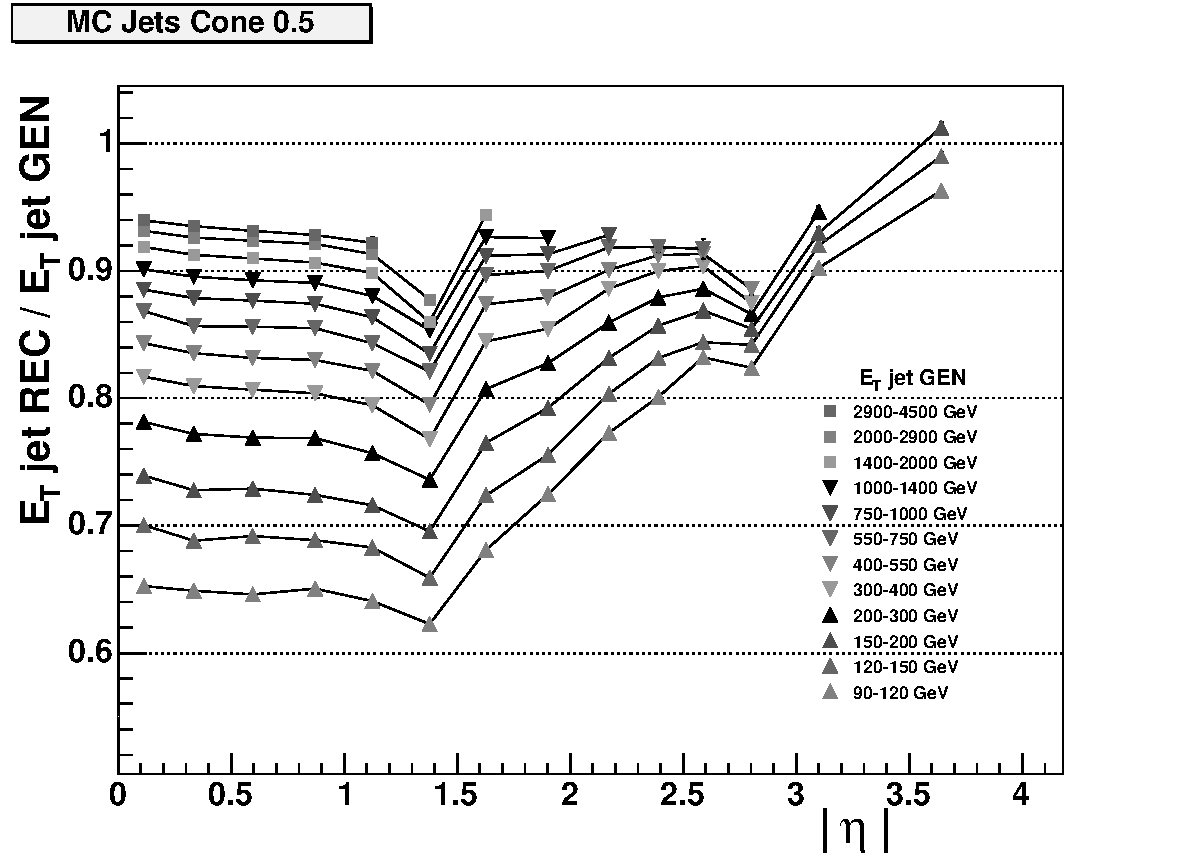
\includegraphics[width=0.8\textwidth]{cms/EtaG_grey}
    \caption{The ratio of the reconstructed jet transverse energy $\mathrm{E_{T}^{rec}}$ 
      to the generated transverse energy \ETMC
      as a function of generated jet $\eta$ for jets with
      different \ETMC reconstructed by the iterative cone
      $R=0.5$ algorithm.~\cite{CMS_TDR_PHYS_vol1}}
    \label{fig:jet_scale}
\end{figure}

\begin{figure}[hbt]
  \centering
  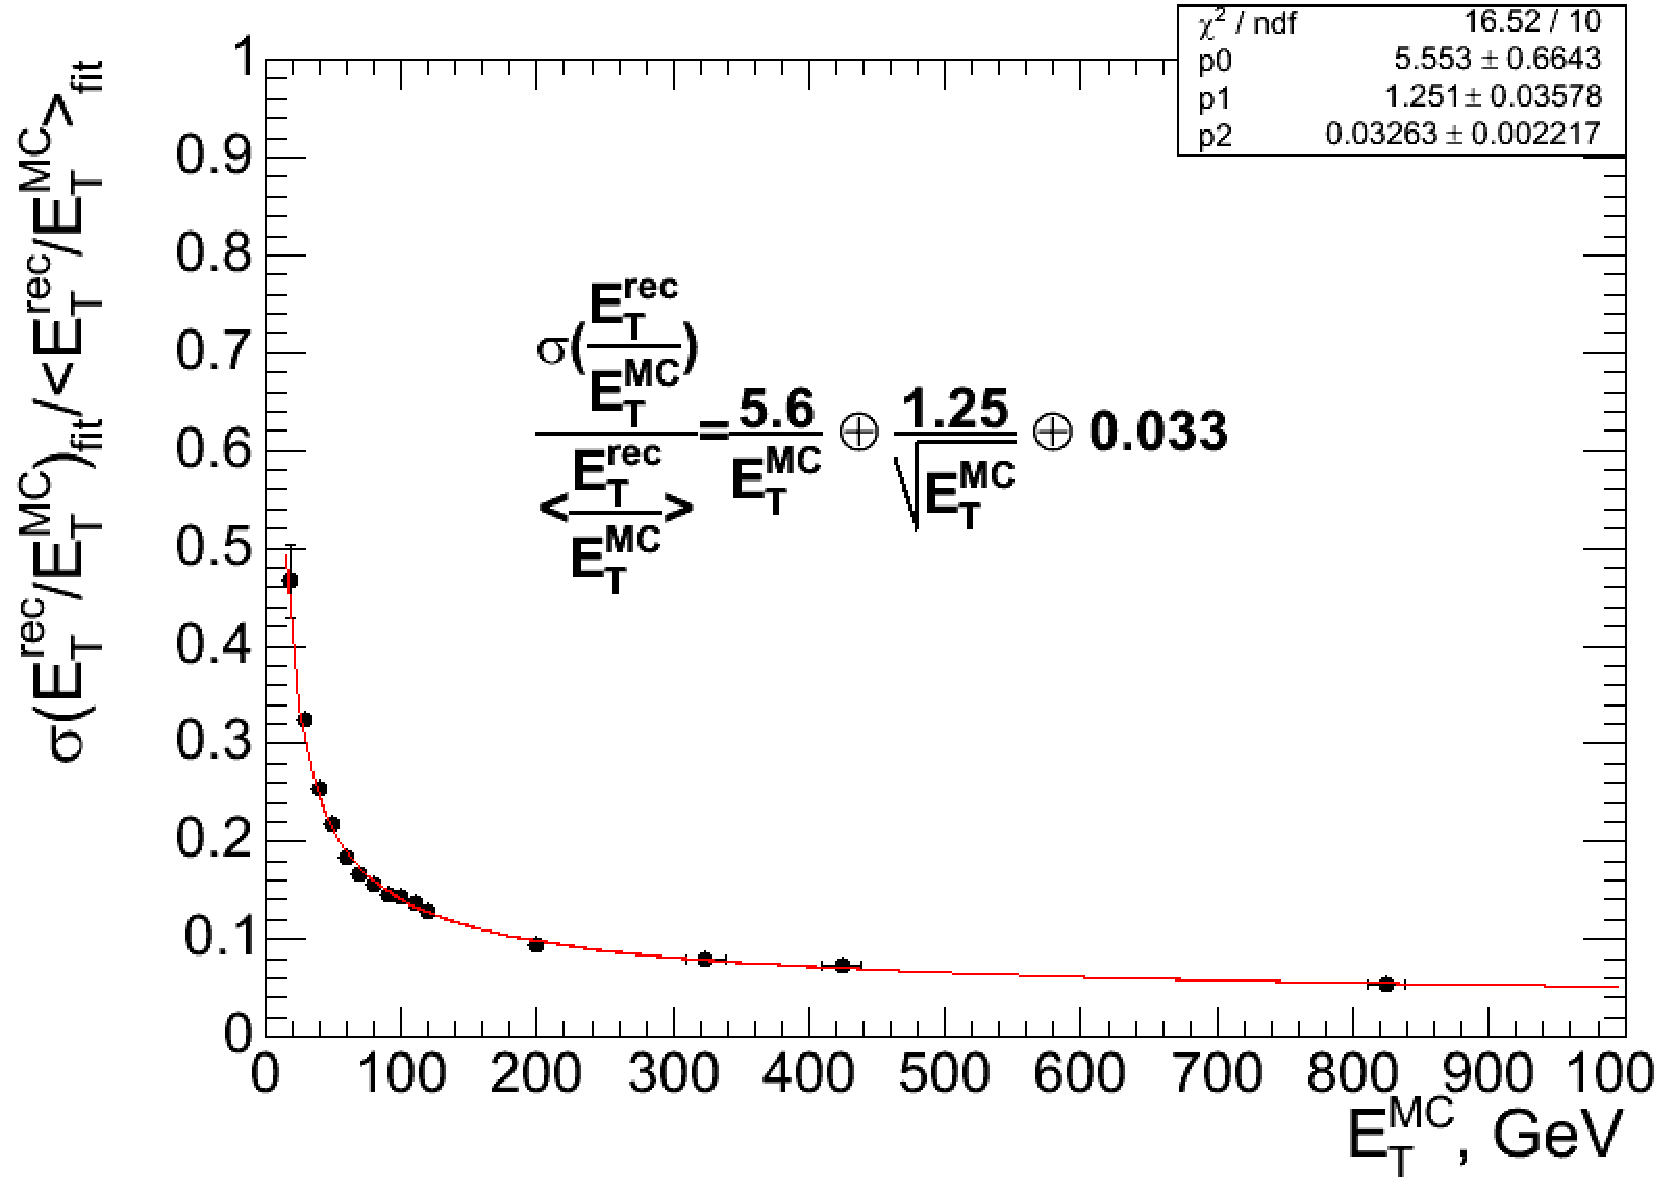
\includegraphics[width=0.8\textwidth]{cms/et_resolution_0508_dr02_bar_cor}
  \caption{The jet transverse energy resolution for simulated jet events with pileup in the HCAL barrel.~\cite{CMS_TDR_PHYS_vol1}
  \label{fig:Jet_perf}}
\end{figure}

The granularity of the different HCAL detectors has been chosen to provide similar jet energy resolutions for all regions. The barrel jet energy resolution can be seen in Figure~\ref{fig:Jet_perf} and can be parameterised: 

\begin{equation}
\mathrm{\frac{\sigma\left(\frac{E_{\rm T}^{\rm rec}}{E_{\rm T}^{\rm MC}}\right)}{\langle\frac{E_{\rm
      T}^{\rm rec}}{E_{\rm T}^{\rm MC}}\rangle}=\frac{5.6}{\ETMC} \oplus
      \frac{1.25}{\ETMC} \oplus 0.033}
\end{equation}

where the first term is the noise term, the second the stochastic term and the third the constant term. The noise is due to fixed energy fluctuations from electronic noise, pileup and the underlying event, the second term is the stochastic calorimeter response and the third is a constant term originating from the non-uniformities and non-linearities of the calorimeter response.

The missing energy \MET mean and resolution distributions for soft ($0 < \PT < 15 \GeV$) QCD dijet events with pile-up are shown in Figure~\ref{fig:MET_perf}. These can be parameterised as:

\begin{equation}
 \langle\MET\rangle \approx 1.25 \sqrt{ \Sigma \ET}
 \label{eqn:MET_mean}
\end{equation}

and

\begin{equation}
 \sigma(\MET)\approx 1.0 \sqrt{ \Sigma \ET}
 \label{eqn:MET_SIGMA}
\end{equation}

\begin{figure}[bt]
  \centering
  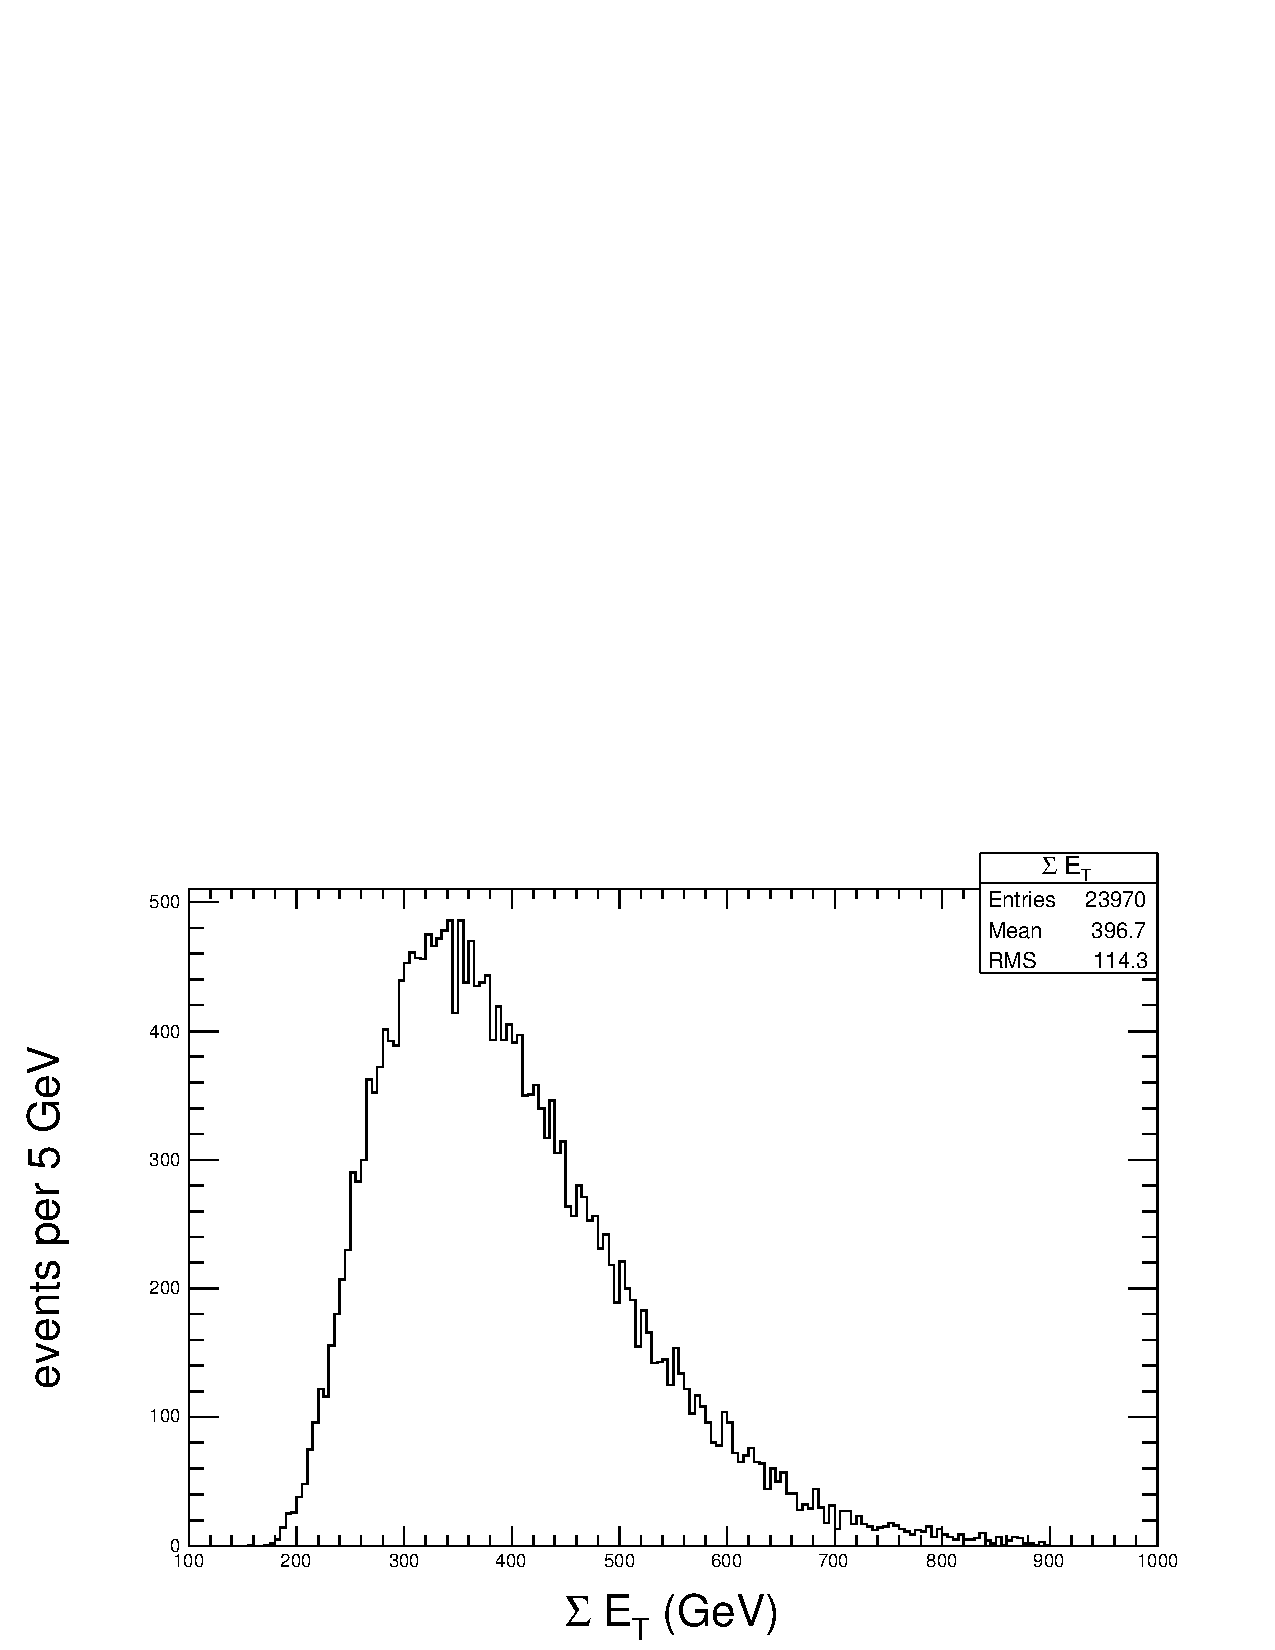
\includegraphics[width=0.45\textwidth]{cms/QCD-0-15-SumEt}
  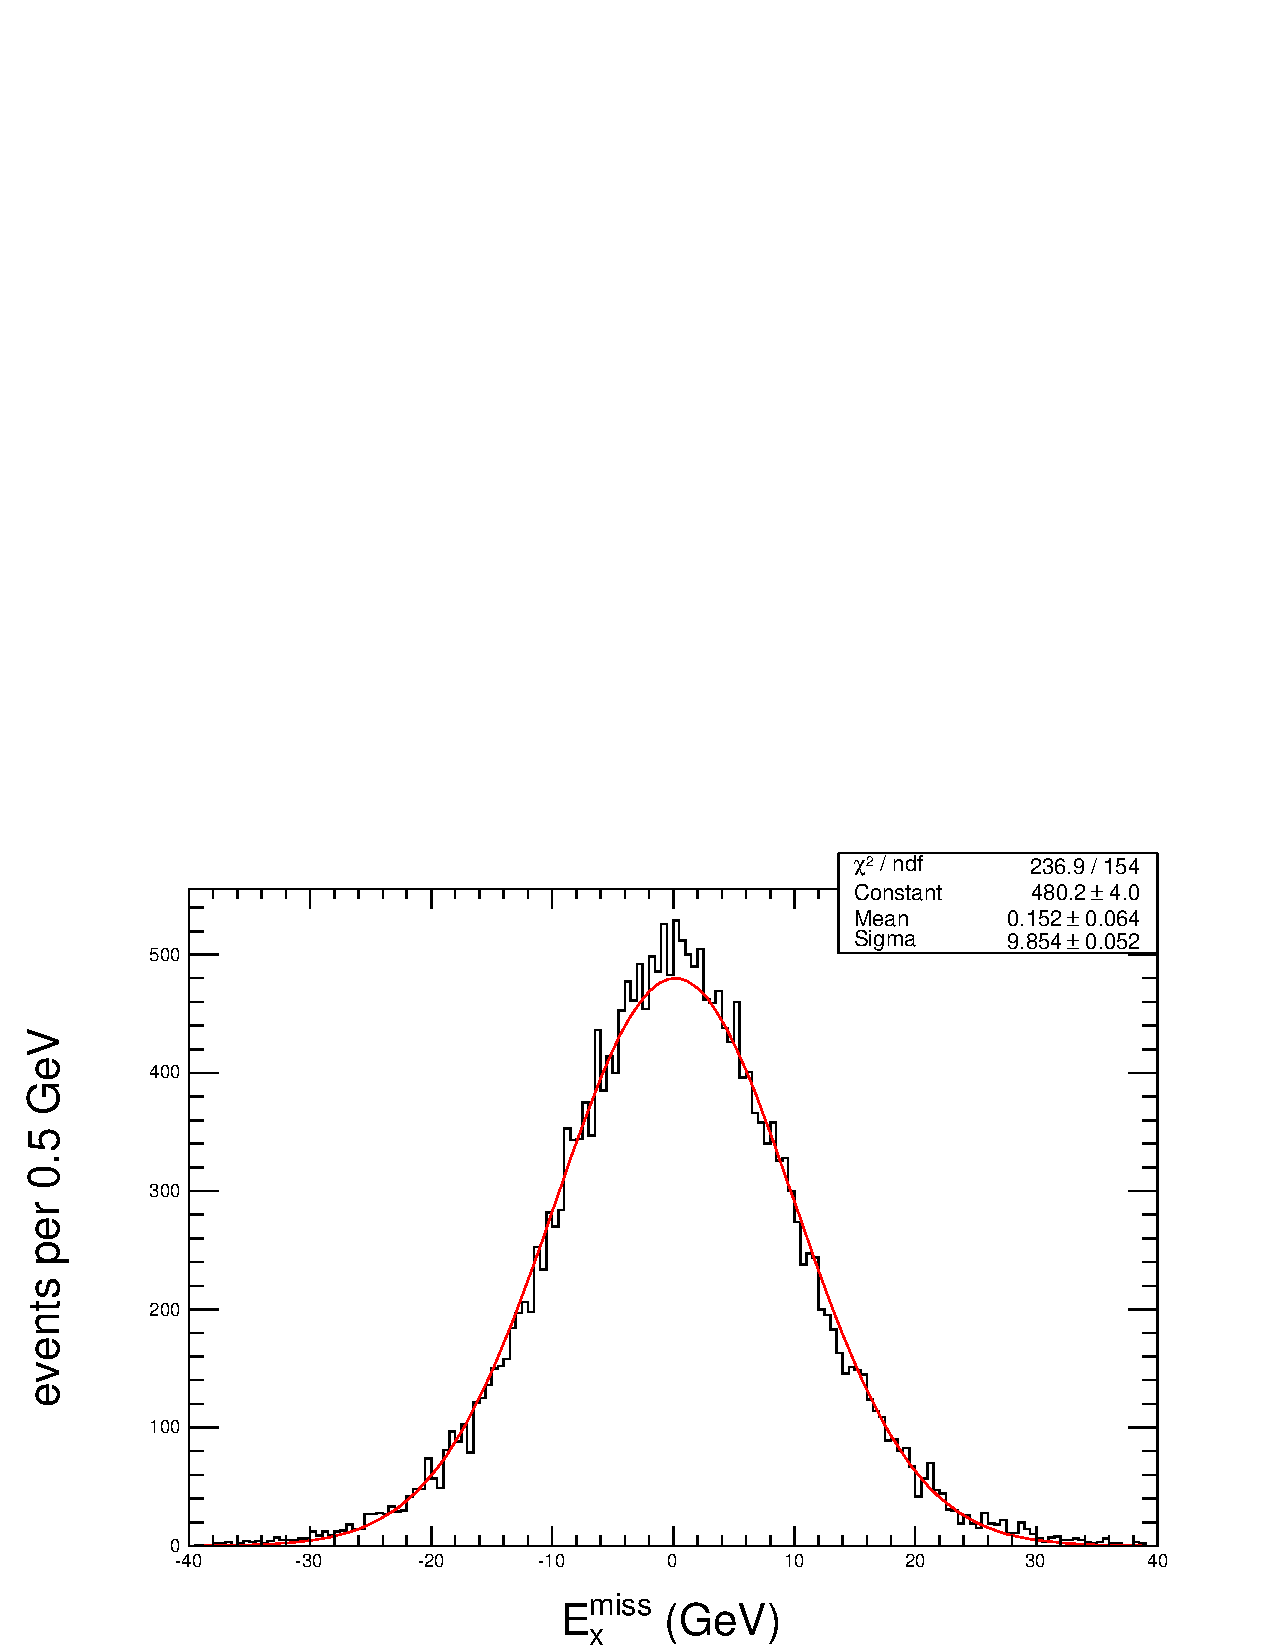
\includegraphics[width=0.45\textwidth]{cms/QCD-0-15-METx}
  \caption{Distribution of sum \ET (left) and $\mathrm{E_{x}^{miss}}$ (right) for soft QCD events with pileup. The \MET resolution of 9.9GeV is in good agreement with Equation~\ref{eqn:MET_SIGMA}.~\cite{CMS_TDR_PHYS_vol1}
  \label{fig:MET_perf}}
\end{figure}

\subsection{The Muon Detectors}
The Muon system provides measurements in the range $|\eta| < 2.4$ and is shown in Figure~\ref{fig:muons}. Detectors are placed at four layers or stations in the barrel and endcap sections of the iron flux return. Three different types of gaseous detector are used due to the varying radiation and magnetic environments. The barrel section, covering $|\eta| < 1.2$, uses drift tubes (DT). The high muon and neutron background environment of the endcaps, $0.8 < |\eta| < 2.4$, means cathode strip chambers (CSC) are used instead of DTs. Resistive Plate Chambers (RPC) are used in both the barrel and part of the endcaps, $|\eta| < 2.1$.

The barrel region contains 250 chambers of up to 12 planes of drift tubes. The individual drift tubes have a cross section of $42 \times 13\,\mmsquare$ and are filled with Ar and $\mathrm{CO_{2}}$. Each drift tube consists of a central anode wire surrounded by aluminum cathodes. The induced charge has a maximum drift length of 2 cm or 400 ns. Each station provides a muon vector with a resolution of 100\micron in $\phi$ and 1 mrad in direction.

The two endcaps use 468 CSCs each of which is trapezoidal and contains 6 gas gaps. Each gap has a plane of radial cathode strips with perpendicular anode wires. The muon position is measured from the charge sharing of the radial cathode strips. Each station provides a muon vector with a resolution of $\sim$200\micron in $\phi$ and 10\,mrad in direction. 

The RPCs consist of a gas gap enclosed by two graphite-coated bakelite plates. The graphite forms a cathode with an aluminum strip used to read out the generated signal. The RPCs have a time resolution of $\sim$1\,ns which makes them useful for identifying the bunch crossing time. 

\begin{figure}[htb]
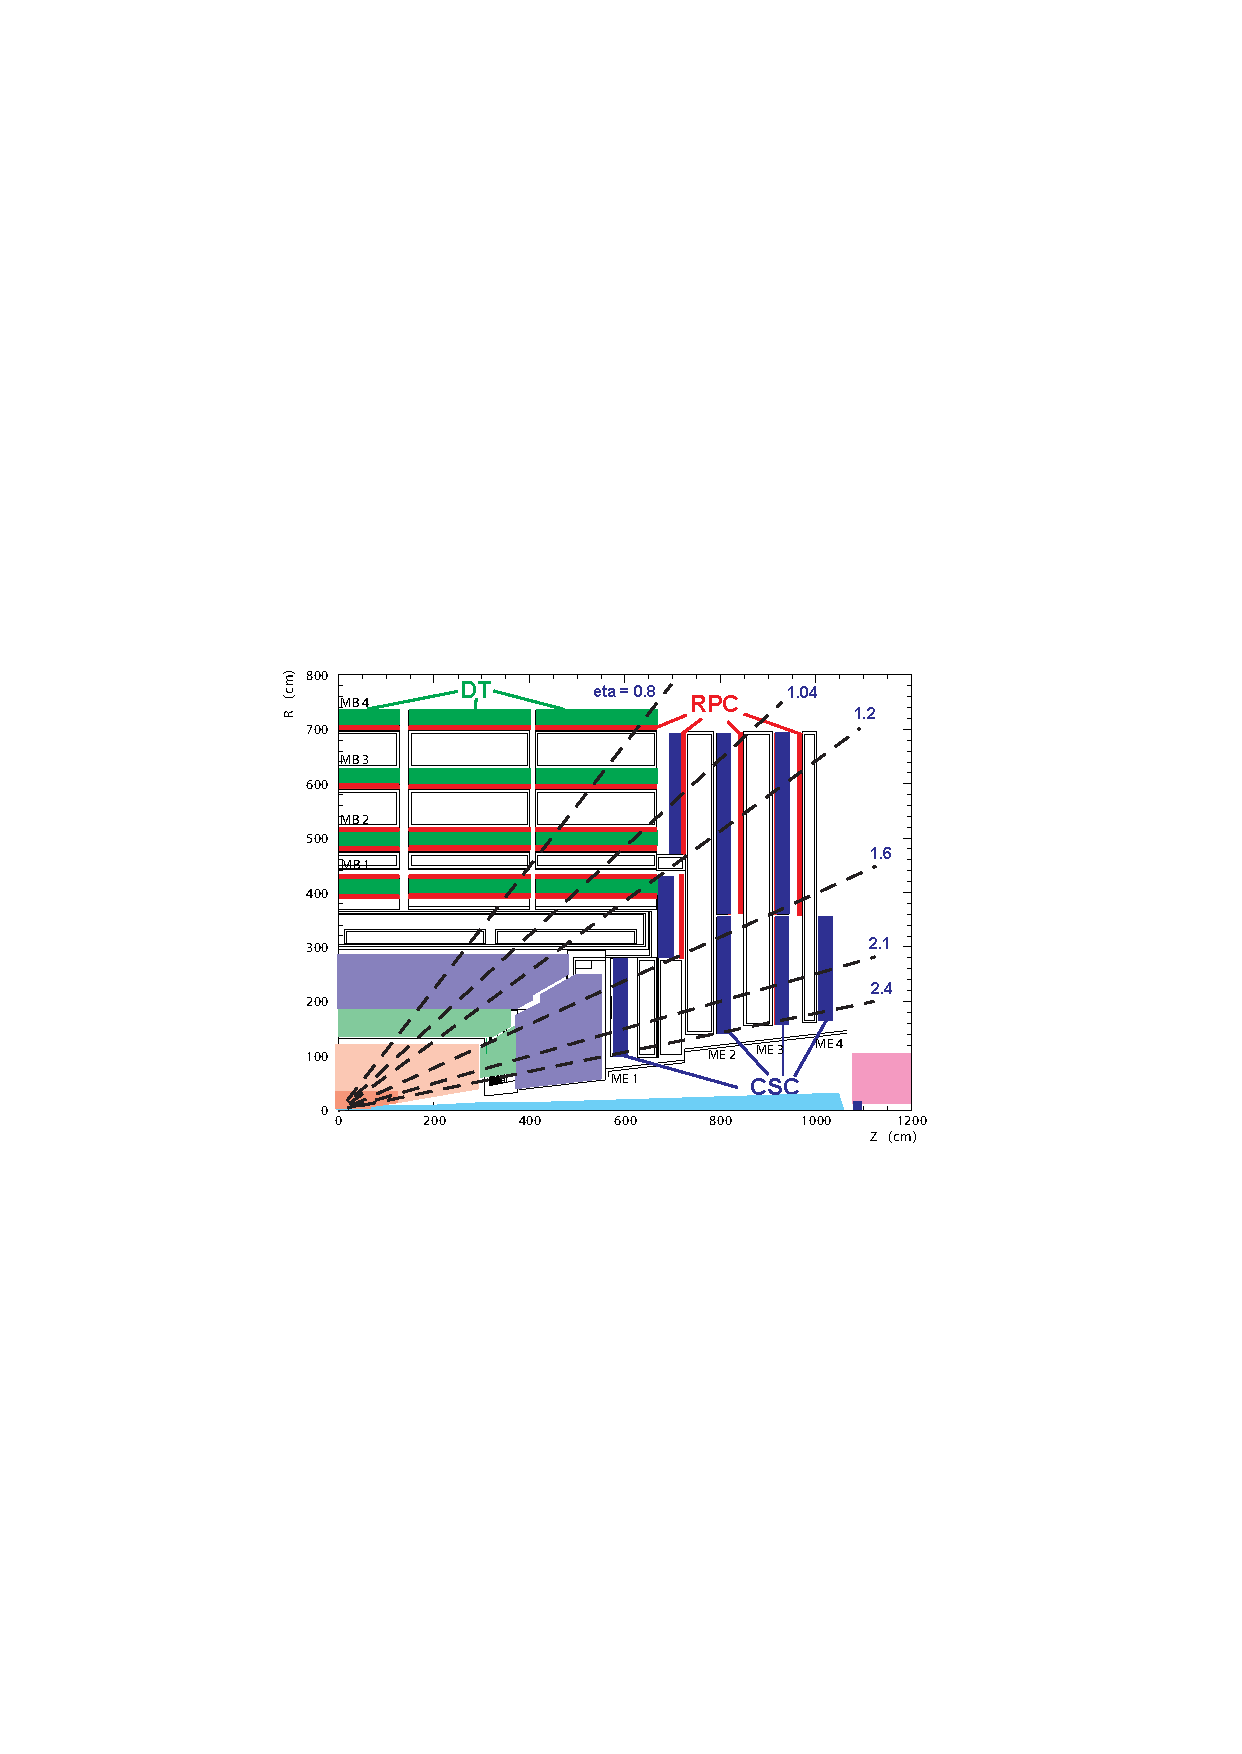
\includegraphics[width=0.9\textwidth]{cms/CMSQuarterView_new}
\caption{Layout of one quarter of the CMS muon system for initial low
luminosity running. The RPC system is limited to $|\eta|<1.6$ in the endcap, and
for the CSC system only the inner ring of the ME4 chambers have been deployed.~\cite{CMS_TDR_PHYS_vol1}
\label{fig:muons}}
\end{figure}

The muon system has a tracking efficiency of over 90\% for 100\GeV muons. The resolution of the muon system, shown in Figure~\ref{fig:muonresol}, is dominated by multiple scattering from the detector materiel in front of the muon detectors. At low momenta the resolution can be improved by using information from the tracker. At higher momenta multiple scattering can be neglected. The muons are then bent in equal and opposite directions before and after the coil, and this can be used at high energies to improve the resolution.

\begin{figure}[tb]
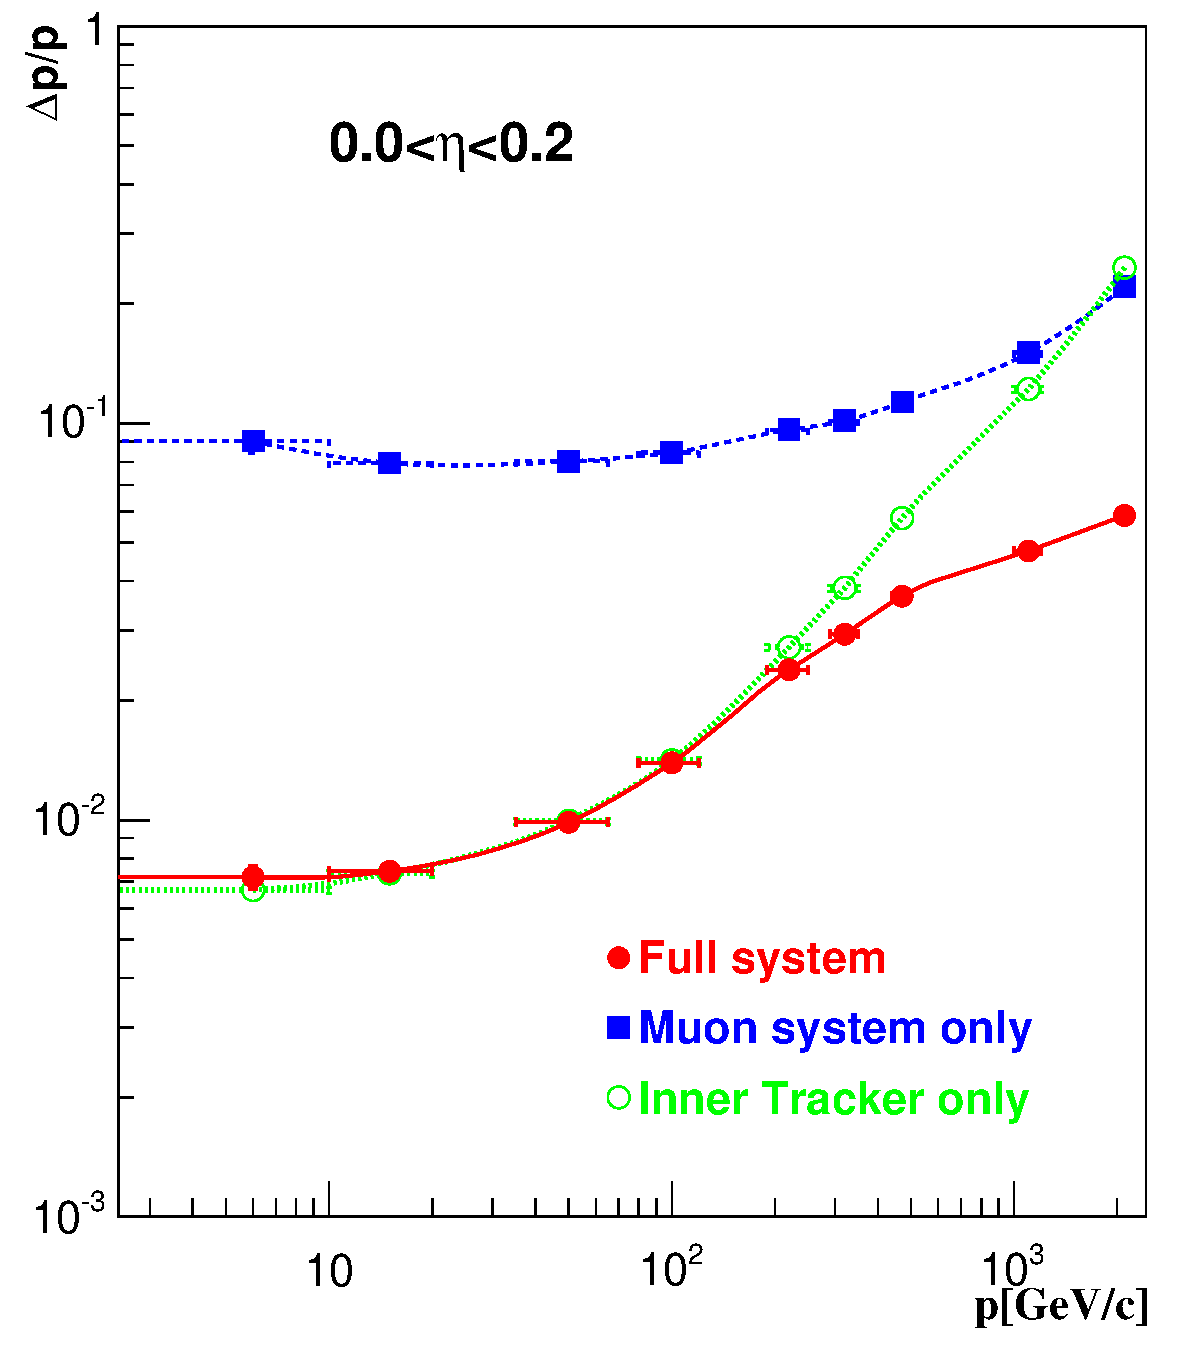
\includegraphics[width=0.48\textwidth]{cms/p_barrel}
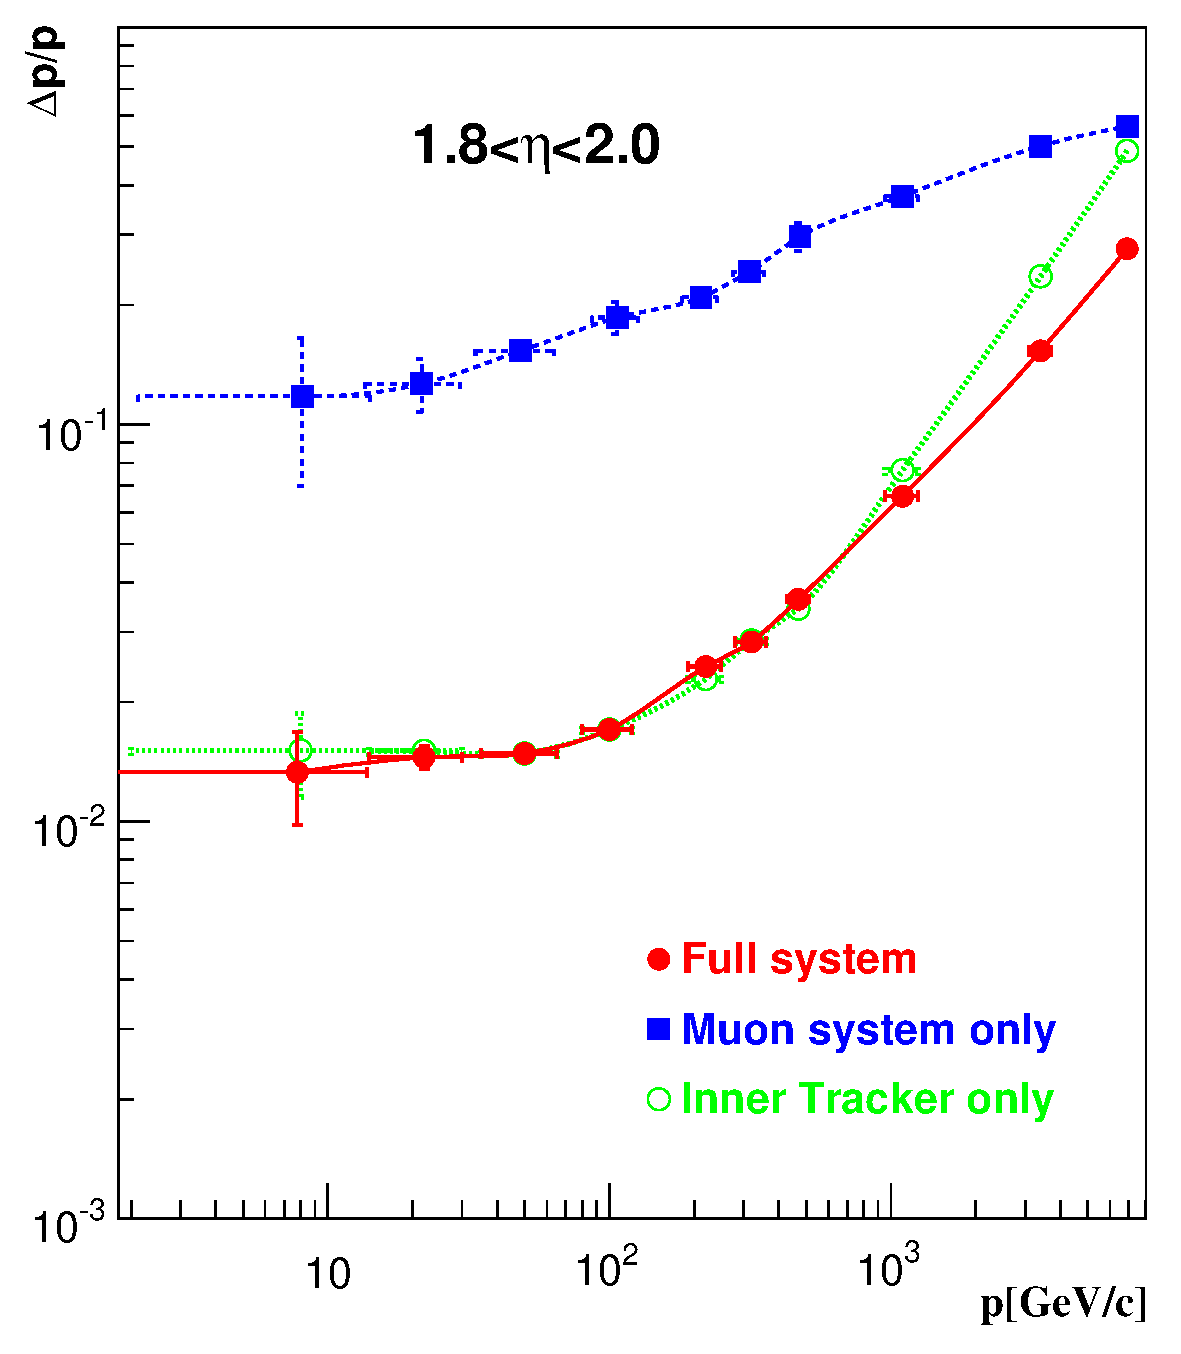
\includegraphics[width=0.48\textwidth]{cms/p_endcaps}
\caption{The muon momentum resolution versus $p$ using the muon
system only, the inner tracker only, or both (``full system''). For the  barrel, $|\eta|<0.2$ (left) and endcap, $1.8<|\eta|<2.0$ (right).~\cite{CMS_TDR_PHYS_vol1}
  \label{fig:muonresol}}
\end{figure}

\subsection{The Trigger System \label{sec:trigger}}
At $\sqrt{s} = 14\TeV$ the proton-proton inelastic cross section is roughly 100 mb. At design luminosity (\hilumi) this results in $10^{9}$ inelastic interactions/s. Given the LHC bunch crossing interval of 25ns (40 MHz), this yields an average of 20 inelastic collisions per bunch crossing (event). Given that CMS has $\sim10^{8}$ detector channels and one event comprises $\sim 1$ MB of data this would give rise to a data rate of 100 TB/s. Storage systems place a limit of 100--200 MB/s, hence an online selection (``trigger'') is used to reduce the event rate to $\sim$100 Hz. 

The CMS trigger is split into two parts; a fast hardware (Level-1) trigger and a software High Level Trigger (HLT). The Level-1 trigger uses custom-built electronics hardware and reduces the event rate from 40 MHz to 100 kHz. The HLT runs on a commodity compute farm and reduces the rate further to $\sim 100$\,Hz for offline storage.

A period of 3.2 $\mu s$ is available for the Level-1 decision, but the signal transit time between the detector and the trigger hardware reduces this to less than 1 $\mu s$. The Level-1 trigger only uses calorimeter and muon information with the rest of the event stored in pipeline memory until the decision is reached.

\begin{figure}[hbt]
  \centering
  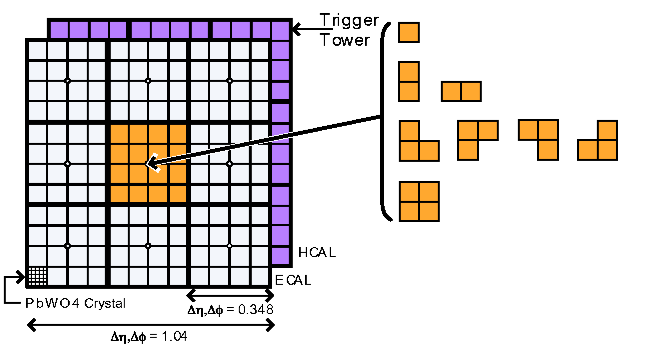
\includegraphics[width=0.5\textwidth]{cms/L1tau}
  \caption{The Level-1 $\tau$ trigger algorithm showing the acceptable $\tau$-like shapes in the central region.~\cite{citeulike:903780}
  \label{fig:L1tau}}
\end{figure}

The Level-1 trigger has separate calorimeter (regional and global) and muon triggers, that are all fed into a global trigger. The regional calorimeter trigger readouts both the ECAL and HCAL calorimetry in coarse grained samples of one HCAL tower or $5\times5$ ECAL barrel crystals, which corresponds to an area of $\Delta\eta \times \Delta\phi = 0.087\times0.087$. The regional calorimeter trigger identifies jet, photon and electron candidates (primitives).

The Level-1 jet trigger sums energy in a $4\times4$ array of towers which are then combined into a $3\times3$ array. Thus a jet is formed from a $12\times12$ array of towers corresponding to approximately a square unit in the $\eta-\phi$ plane. Separate lists are made of central and forward jets. The Level-1 $\tau$ algorithm (Figure~\ref{fig:L1tau}), is similar to the jet algorithm but requires an isolated narrow energy deposit in the central $4\times4$ tower array.  

The Global Calorimeter Trigger (GCT) combines the information from the regional calorimeter triggers and creates an \ET ordered list of each primitive type. The global Level-1 trigger combines the information from the GCT and muon trigger and uses threshold cuts on the primitives to make the accept/reject decision. 

Once accepted by the Level-1 trigger the event is readout and combined by an event builder via a switched network capable of a data transmission rate of 1 TB/s. Once combined the event is sent to a processor in the compute farm, which runs the HLT algorithms and makes the accept/reject decision. Scalability of the system is ensured with the addition of additional event builders and processor units which use the high speed network to communicate. As such during the low luminosity phase only a fraction of the total system will be implemented. As the data rate increases more event builders and processing nodes will be added.

By using a pure software high level trigger maximum flexibility of the reconstruction and triggering criteria can be achieved. The HLT rejects events as soon as possible by using the minimum of event information and by performing partial event reconstruction. Full granularity calorimeter information is used, followed by the tracker pixel detector and finally the full event is reconstructed using all detectors. If an event passes the HLT it is passed to the offline computing system together with a list of all primitives that passed the thresholds, the trigger bits.
